% Created 2026-05-04 Mon 14:02
% Intended LaTeX compiler: lualatex
\DocumentMetadata{lang = en-US,pdfversion = 2.0,pdfstandard = ua-2,tagging = on,tagging-setup = {math/setup=mathml-SE},}
\documentclass[11pt]{article}
\usepackage{amsmath}
\usepackage{fontspec}
\usepackage{graphicx}
\usepackage{longtable}
\usepackage{wrapfig}
\usepackage{rotating}
\usepackage[normalem]{ulem}
\usepackage{capt-of}
\usepackage{hyperref}
\usepackage[margin=1in]{geometry}
\usepackage{fontspec}
\usepackage{verbatim, multicol, tabularx,}
\usepackage{amsmath, amsthm, amssymb, stmaryrd, latexsym, bm, listings, qtree}
\usepackage{framed}
\usepackage{xcolor,colortbl}
\usepackage{media9}
\usepackage[export]{adjustbox}
\usepackage{algorithm}
\usepackage[noend]{algpseudocode}
\usepackage{tikz,pgfplots}
\usetikzlibrary{shapes.geometric}
\let\oldquote=\quote
\let\endoldquote=\endquote
\colorlet{shadecolor}{cyan!15}
\renewenvironment{quote}{\begin{shaded*}\begin{oldquote}}{\end{oldquote}\end{shaded*}}
% From https://tex.stackexchange.com/questions/7032/good-way-to-make-textcircled-numbers
\newcommand*\circled[1]{\tikz[baseline=(char.base)]{\node[shape=circle,draw,inner sep=2pt] (char) {#1};}}
\DeclareMathOperator*{\argmin}{arg\!min}
\DeclareMathOperator*{\argmax}{arg\!max}
\lstset{frame=tb, aboveskip=1mm, belowskip=0mm, showstringspaces=false, columns=flexible, basicstyle={\scriptsize\ttfamily}, numbers=left, frame=single, breaklines=true, breakatwhitespace=true}
\hypersetup{colorlinks=true,urlcolor=blue}
\usepackage{tagpdf}
\tagpdfsetup{activate-all}
\tagpdfsetup{math/alt/use}
\usepackage{polyglossia}
\setdefaultlanguage[variant=en-US]{english}
\author{Christopher Simpkins}
\date{Kennesaw State University}
\title{Reinforcement Learning\\\medskip
\large Temporal-Difference Learning (RLbook 6)}
\hypersetup{
 pdfauthor={Christopher Simpkins},
 pdftitle={Reinforcement Learning},
 pdfkeywords={},
 pdfsubject={Reinforcement Learning - Temporal-Difference Learning (RLbook 6)},
 pdfcreator={Emacs 30.2 (Org mode 9.7.11)}, 
 pdflang={English}}
\begin{document}

\maketitle
\section{Temporal-Difference Learning}
\label{sec:org9f403b8}

\begin{itemize}
\item DP Review

\begin{itemize}
\item Dynamic programming
\item Generalized policy iteration (GPI)
\end{itemize}

\item Model-free control

\begin{itemize}
\item Monte Carlo control
\item Temporal-difference learning
\end{itemize}
\end{itemize}
\section{Dynamic Programming}
\label{sec:org8fcf66c}

Dynamic programming algorithms, as well as RL algorithms in general, contain two phases (combined in value iteration):

\begin{itemize}
\item Prediction: estimate the value function
\item Control: computing or approximating optimal policies
\end{itemize}



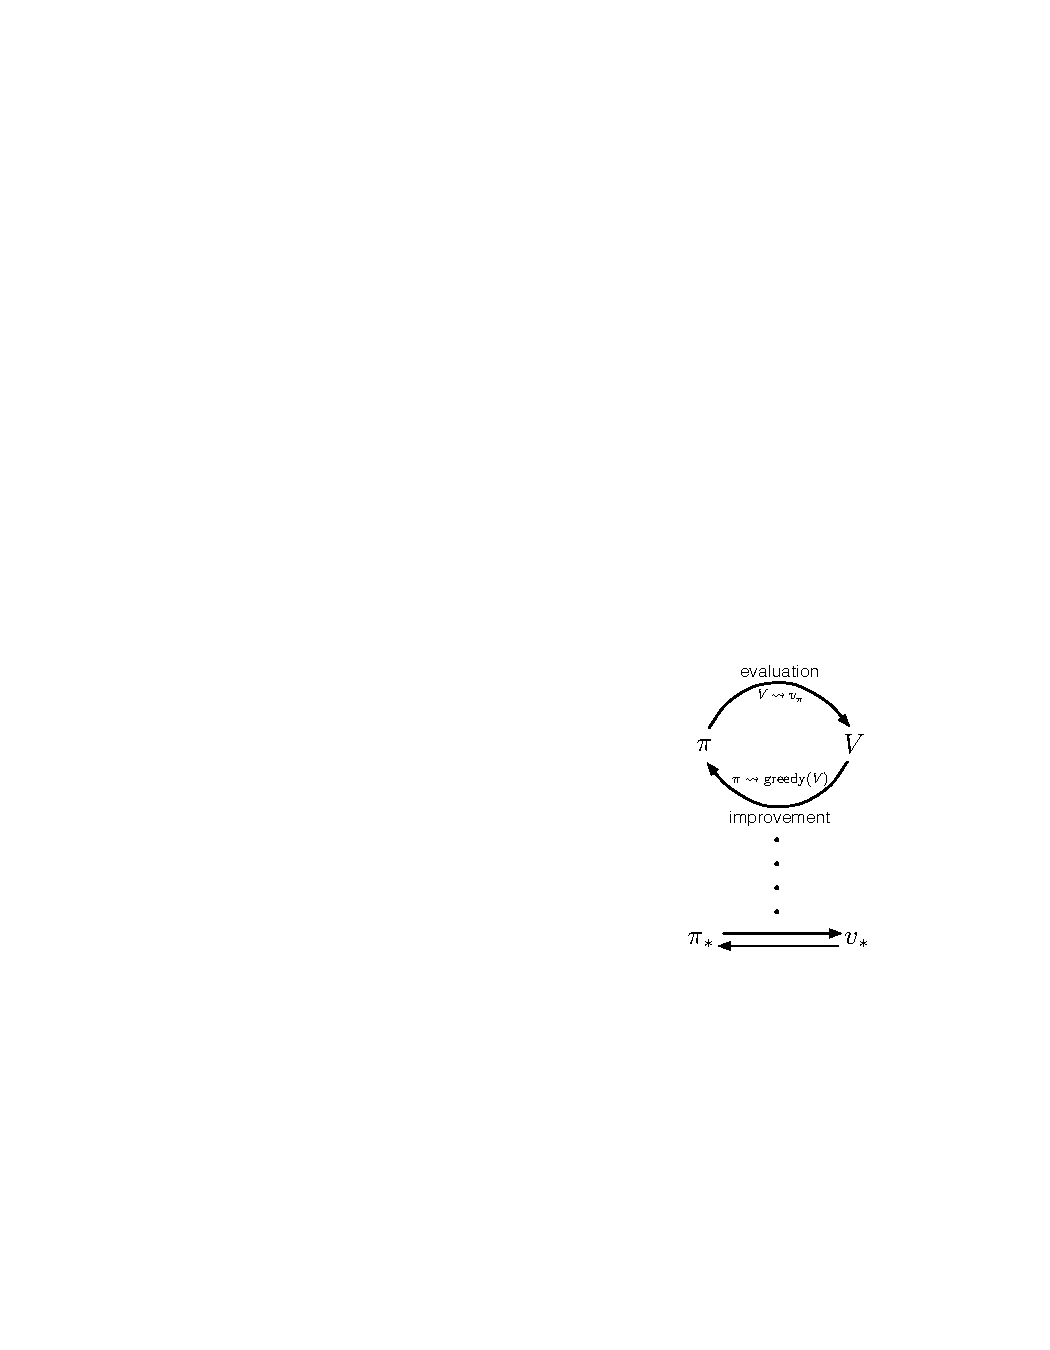
\includegraphics[alt={rlbook 04 09 value policy evaluation improvement loop},width=0.5\linewidth]{rlbook-04-09-value-policy-evaluation-improvement-loop.pdf}
\section{Generalized Policy Iteration}
\label{sec:orgbd8fe1a}

In policy iteration we sweep entire state space in each step.


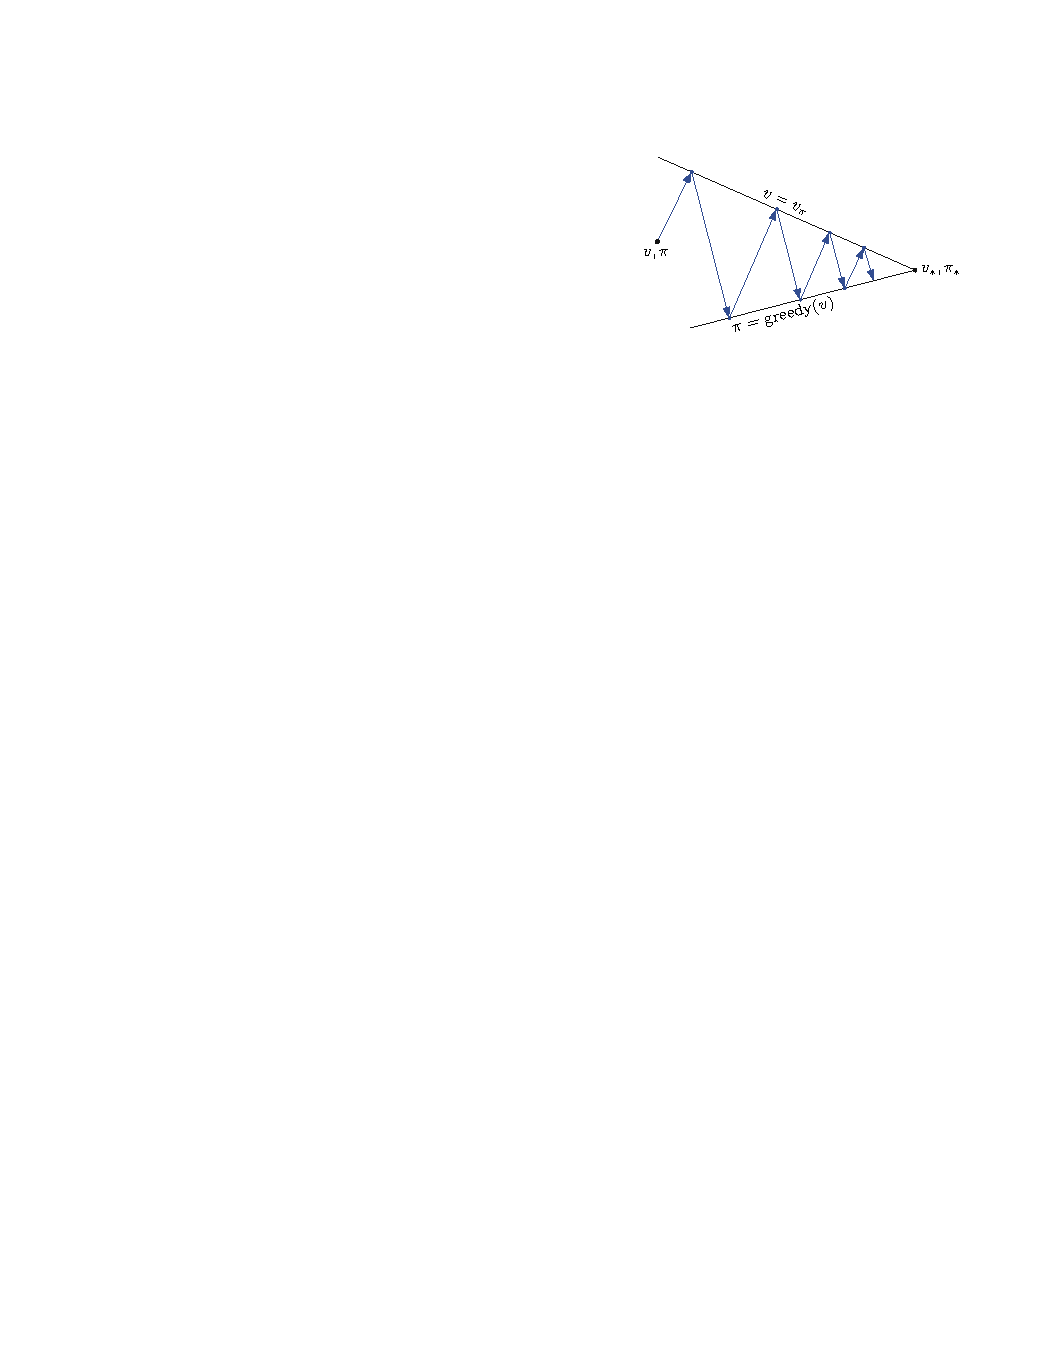
\includegraphics[alt={rlbook 04 10 value policy convergence diagram},width=0.75\linewidth]{rlbook-04-10-value-policy-convergence-diagram.pdf}


In generalized policy iteration (GPI) we interleave prediction and control at arbitrary granularity.

\begin{itemize}
\item As long as we visit every state, still assured of convergence.
\end{itemize}

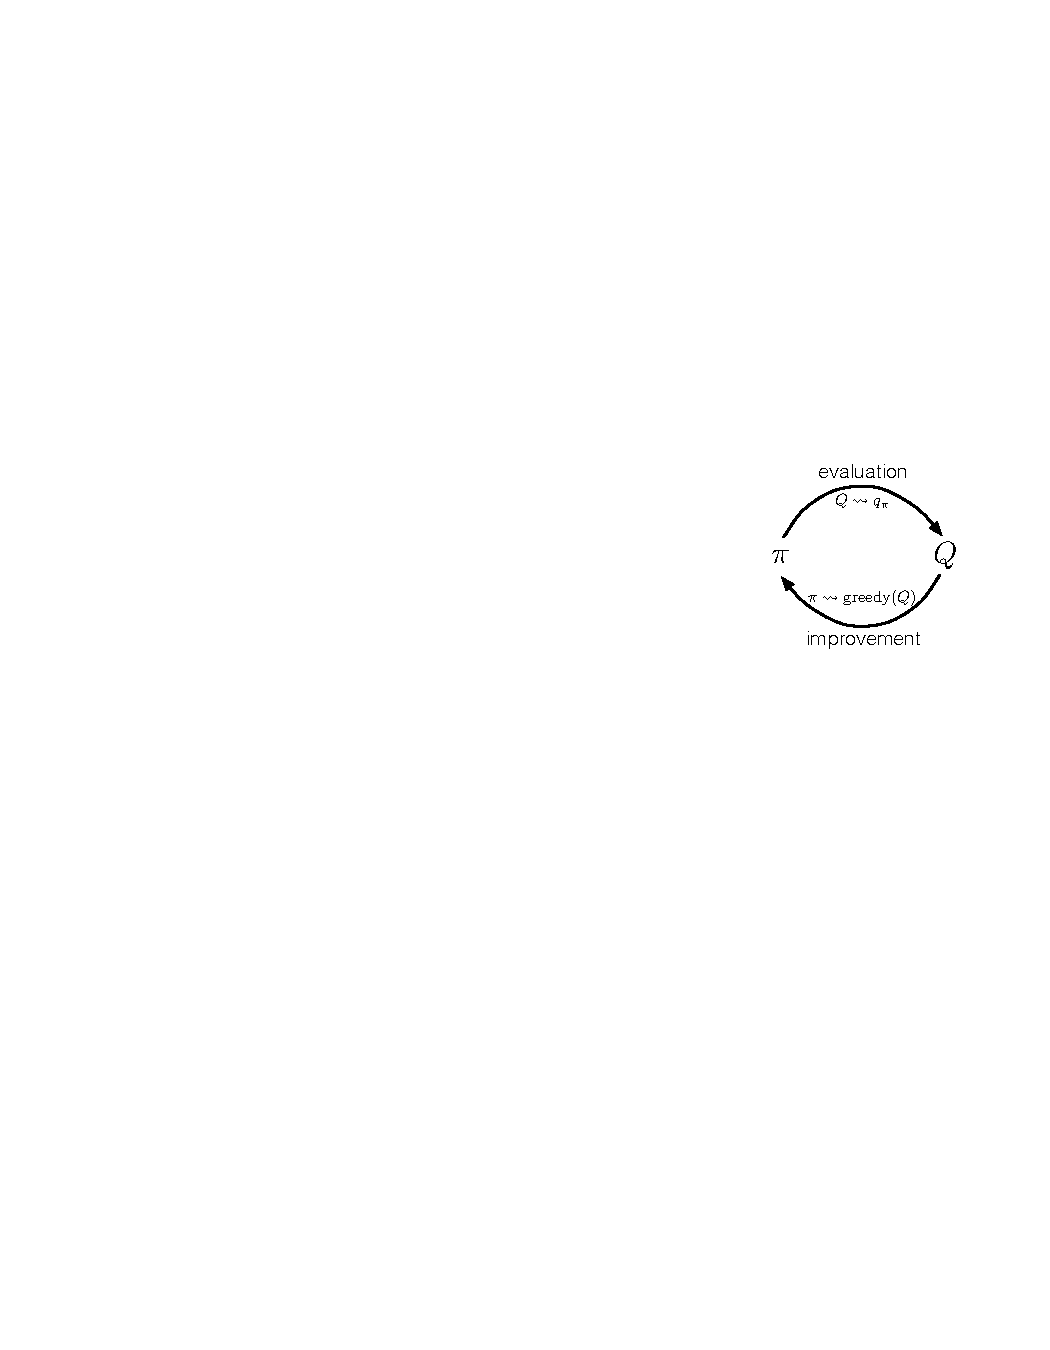
\includegraphics[alt={rlbook 05 05 evaluation improvement loop},width=0.75\linewidth]{rlbook-05-05-evaluation-improvement-loop.pdf}
\section{Monte Carlo Methods}
\label{sec:org53da88a}

Monte Carlo methods sample and average returns for each state–action pair.

\begin{itemize}
\item Generate a set of episode samples by following a policy \(\pi\)
\item For each visit to a state \(s\), find the first visit to \(s\), then average all the returns following the first visit to \(s\) to estimate the value of \(s\)
\end{itemize}

\includegraphics{[}alt=\{rlbook 05 03 monte carlo full trajectory backup\},width=1in]\{rlbook-05-03-monte-carlo-full-trajectory-backup.pdf\}
\section{Temporal-Difference Learning}
\label{sec:orgf621441}

Combination of dynamic programming and Monte Carlo ideas.

\begin{itemize}
\item Like Monte Carlo, learn directly from experience without a model of the environment.
\item Like dynamic programming, update estimates based in part on other learned estimates, without waiting for a final outcome (bootstrap).
\end{itemize}
\section{TD Prediction}
\label{sec:orgd78248d}

Use experience following a policy to update estimate of \(V\), namely \(v_{pi}\).

Monte Carlo methods wait until the return following the visit is known, then use that return as a target for \(V(S_t)\):

\begin{equation*}
V (S_t) \gets V (S_t) + \alpha \left[ G_t - V(S_t) \right] \tag{6.1}
\end{equation*}

TD methods only until the next time step. At time \(t + 1\) they immediately form a target and make a useful update using the observed reward \(R_{t+1}\) and the estimate \(V(S_{t+1})\)

A simple TD method makes the update:

\begin{equation*}
V (S_t) \gets V (S_t) + \alpha \left[ R_{t+1} + \gamma V(S_{t+1}) - V(S_t) \right]
\end{equation*}

immediate on transition to \(S_{t+1}\) and receiving \(R_{t+1}\).

\begin{itemize}
\item Target for Monte Carlo update is \(G_t\).
\item Target for TD update is \(R_{t+1} + \gamma V(S_{t+1})\)
\end{itemize}
\section{Tabular TD(0) Algorithm}
\label{sec:orgb28d57c}

One-step TD is called \(TD(0)\), which is a special case of \(TD(\lambda)\) and \$n\$-step methods.


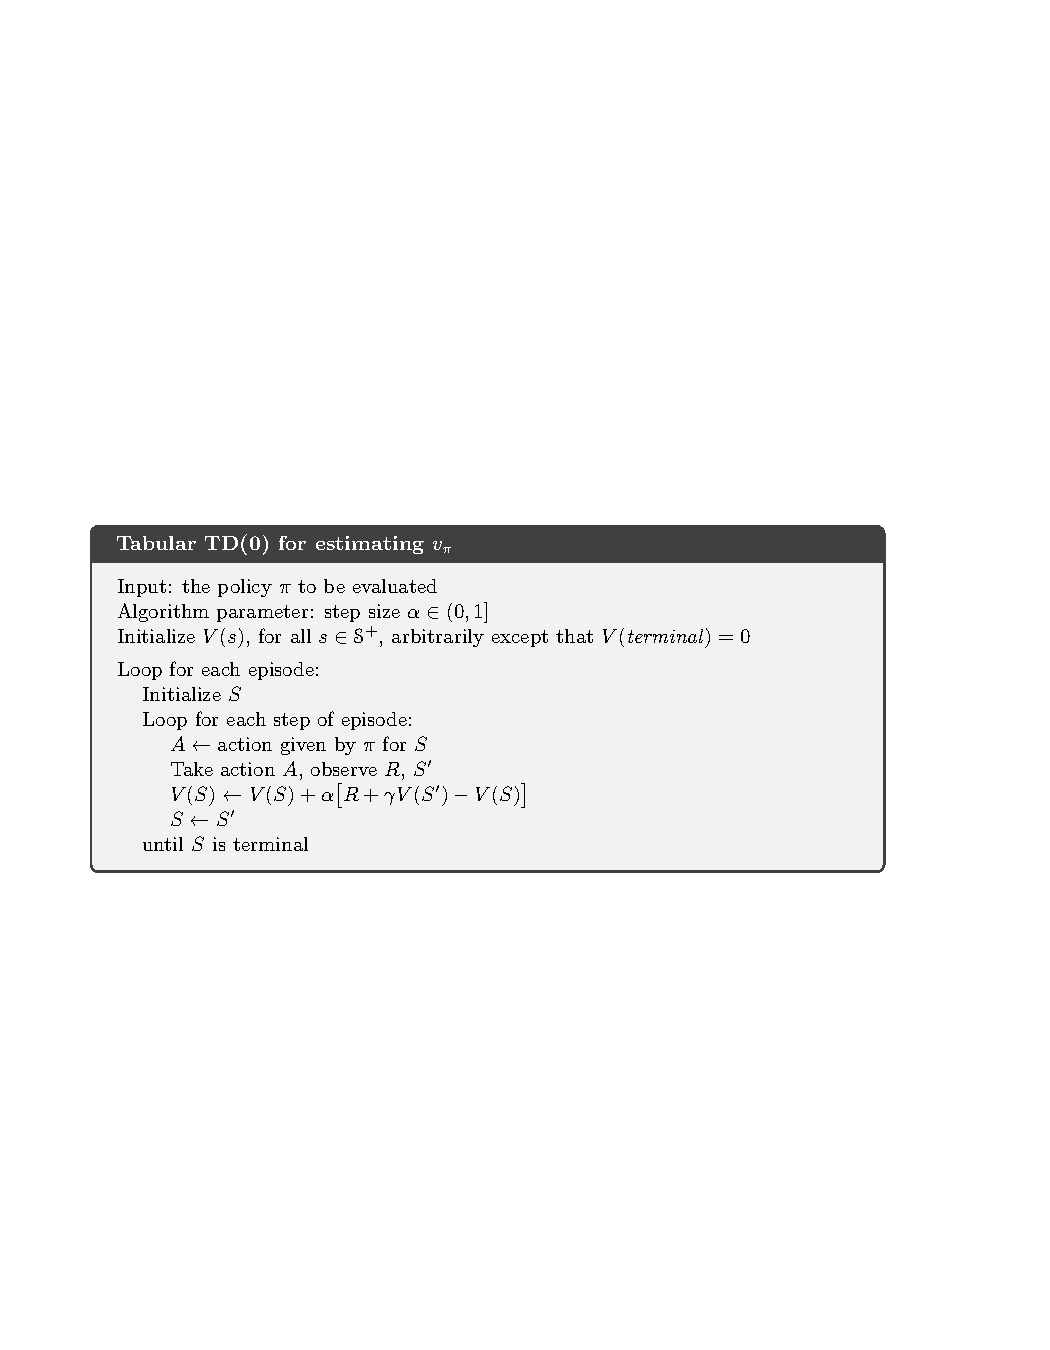
\includegraphics[alt={rlbook 06 01 tabular td0 algorithm},width=0.75\linewidth]{rlbook-06-01-tabular-td0-algorithm.pdf}
\section{TD Error}
\label{sec:orgcb29ec2}




Recall TD update:

\begin{equation*}
V (S_t) \gets V (S_t) + \alpha \left[ R_{t+1} + \gamma V(S_{t+1}) - V(S_t) \right]
\end{equation*}

The quantity in brackets is called \textbf{TD error} -- the difference in the estimate value of \(S\) at time \(t\) and \(t+1\):

\begin{equation*}
\delta \doteq R_{t+1} + \gamma V(S_{t+1}) - V(S_t)
\end{equation*}



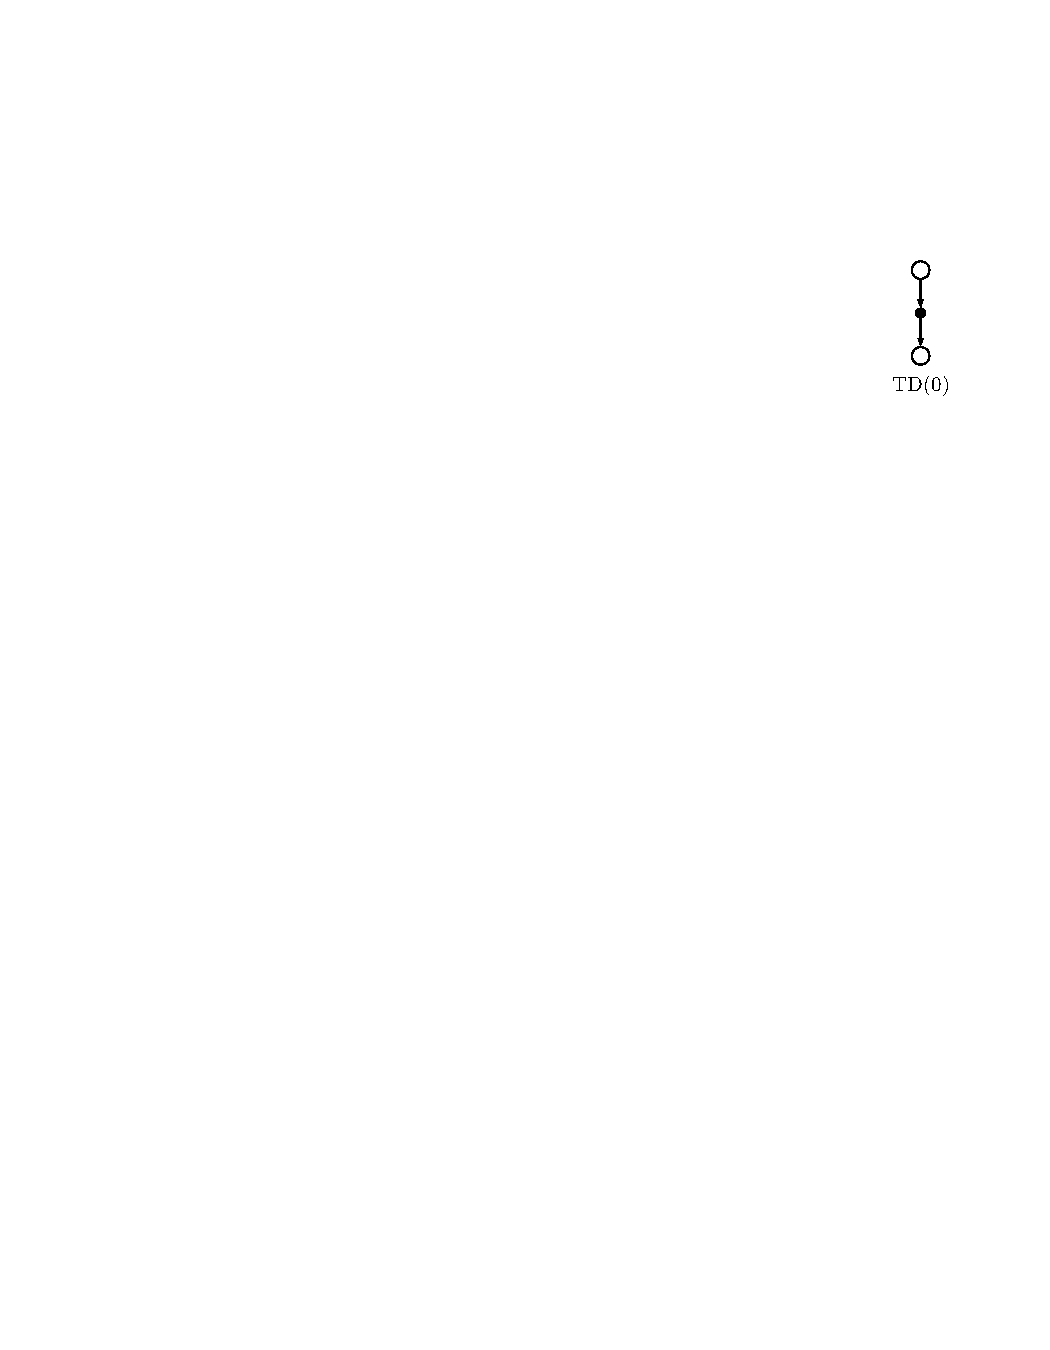
\includegraphics[alt={rlbook 06 02 td0 backup},width=0.75in]{rlbook-06-02-td0-backup.pdf}
\section{Sarsa: On-policy TD Control}
\label{sec:orgebf7a1c}


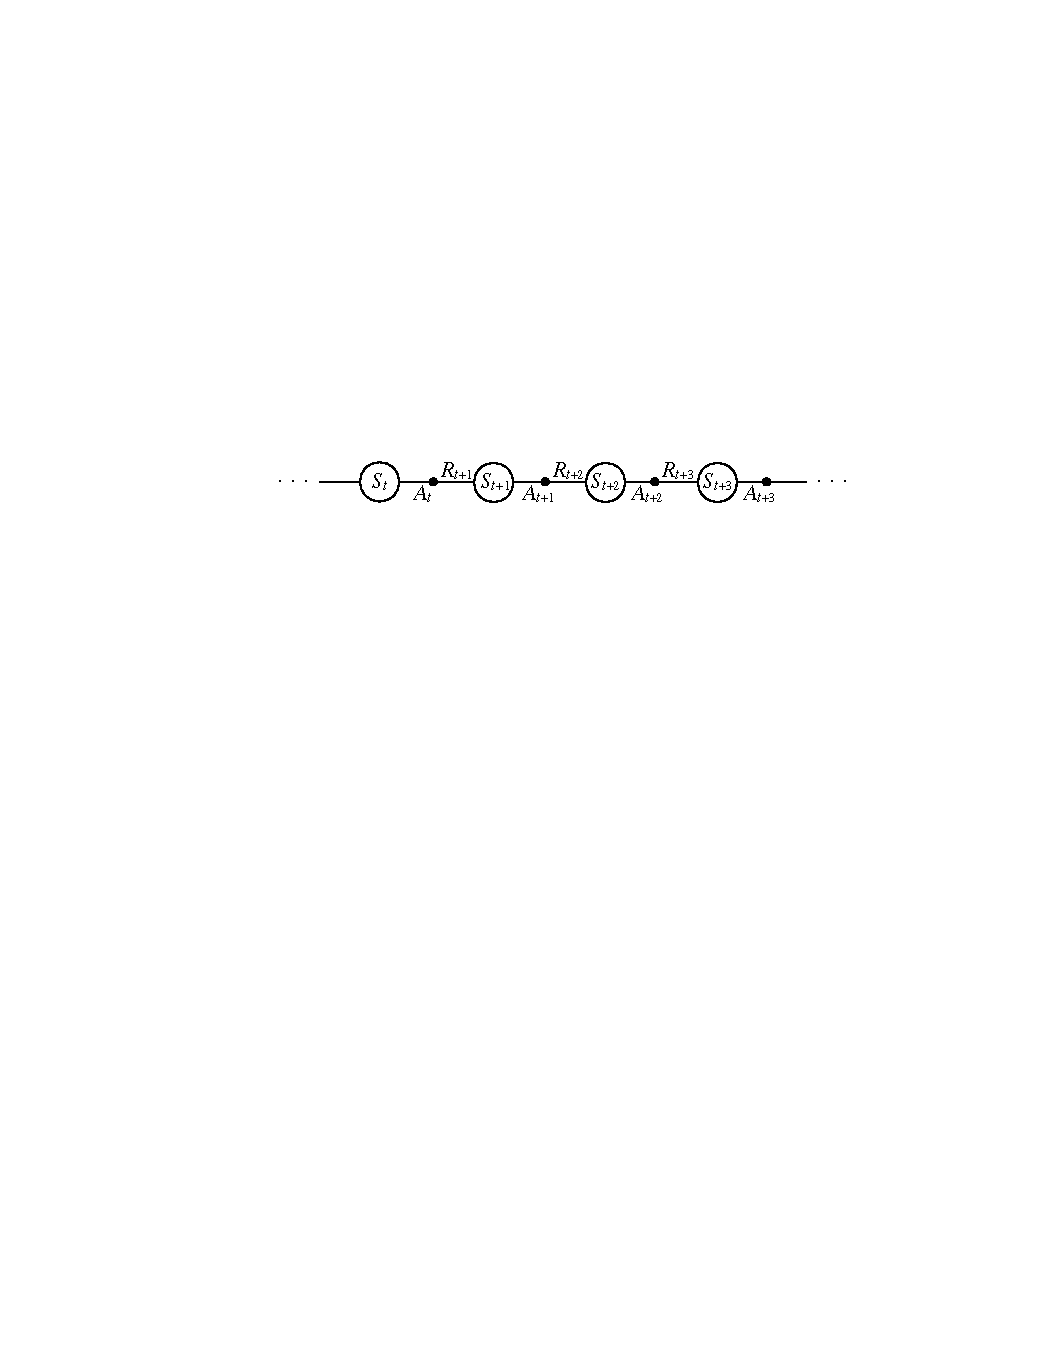
\includegraphics[alt={rlbook 06 09 episode state action sequence diagram},width=0.75\linewidth]{rlbook-06-09-episode-state-action-sequence-diagram.pdf}


Sarsa update:

\begin{equation*}
Q(s_t, a_t) \gets Q(s_t, a_t) + \alpha \left[ R_{t+1} + \gamma Q(s_{t+1}, a_{t+1}) - Q(S_t, A_t) \right]
\end{equation*}


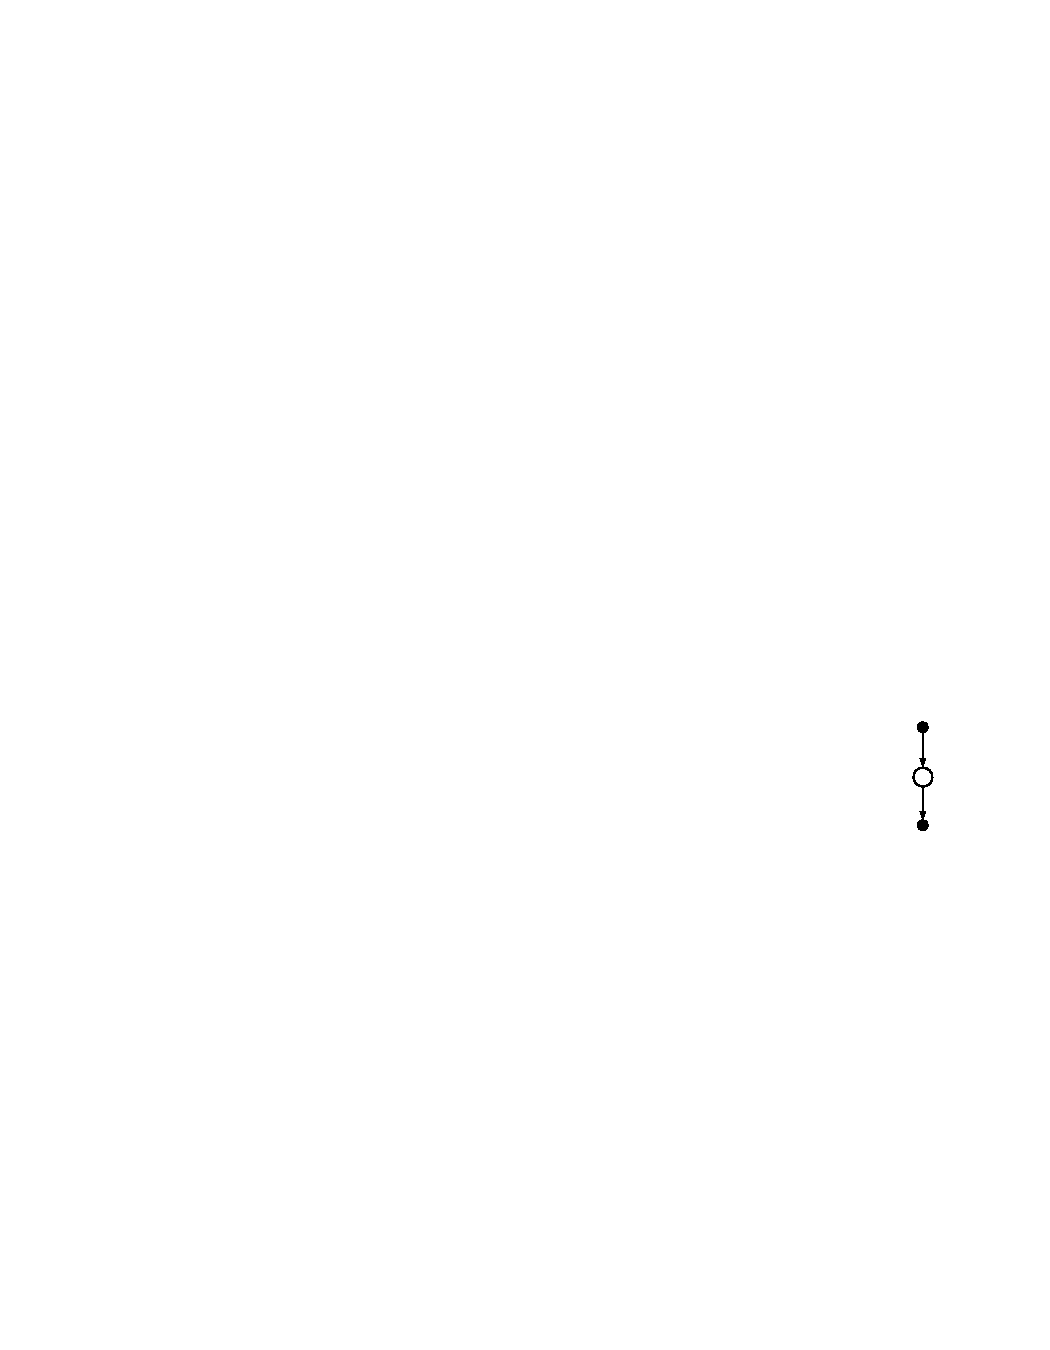
\includegraphics[alt={rlbook 06 10 sarsa backup diagram},width=0.75in]{rlbook-06-10-sarsa-backup-diagram.pdf}
\section{Sarsa Algorithm}
\label{sec:org64731b3}


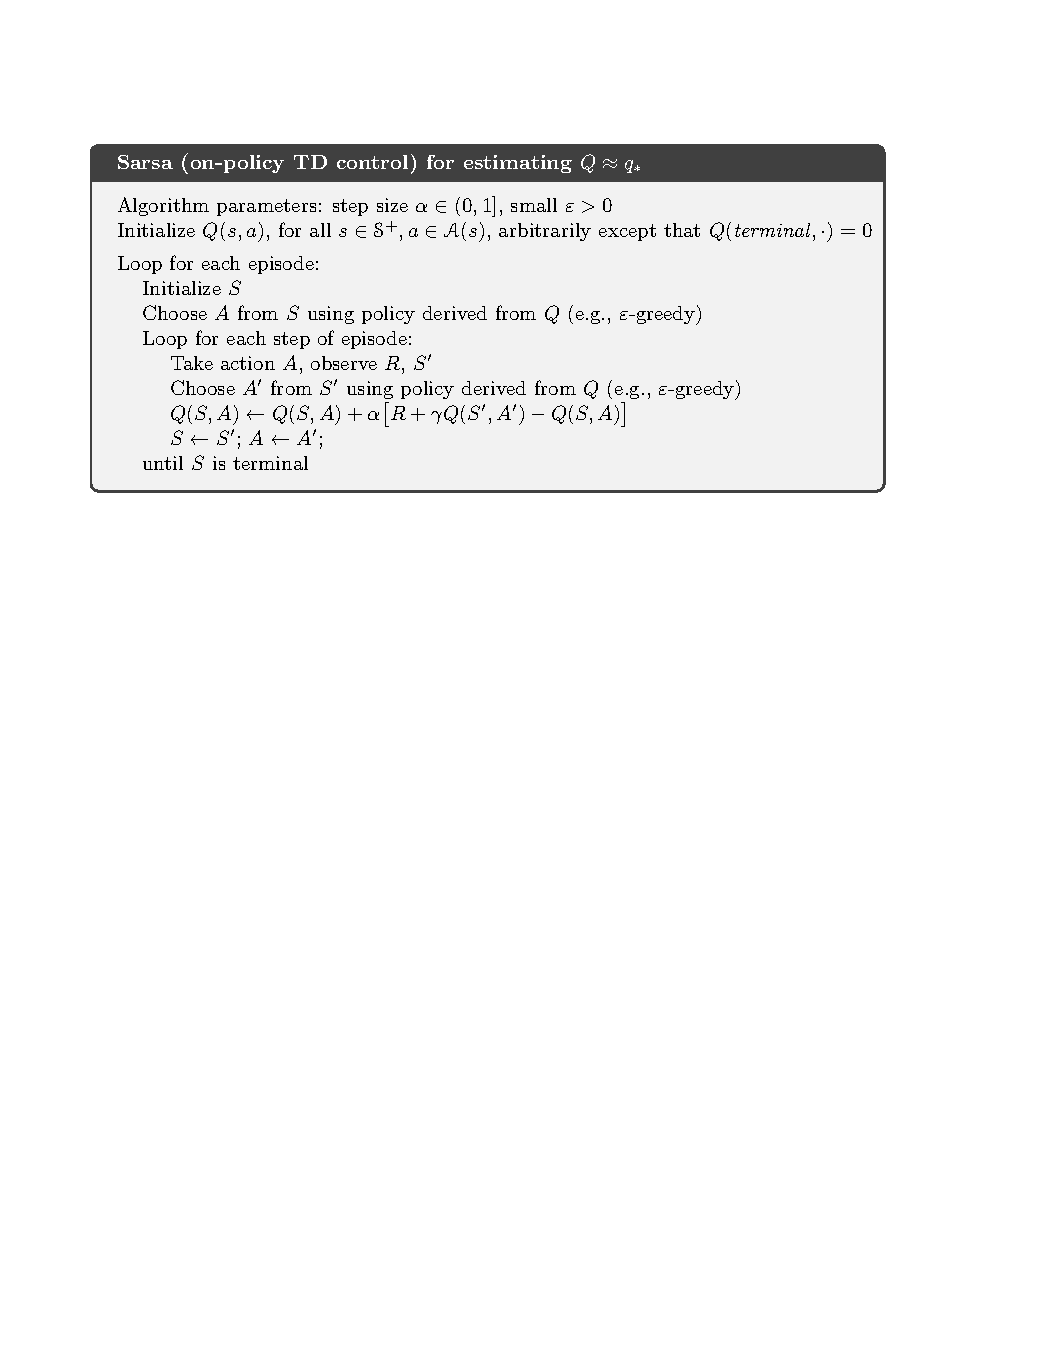
\includegraphics[alt={rlbook 06 11 sarsa algorithm},width=0.9\linewidth]{rlbook-06-11-sarsa-algorithm.pdf}
\section{Example: Windy Grid World}
\label{sec:org3943028}


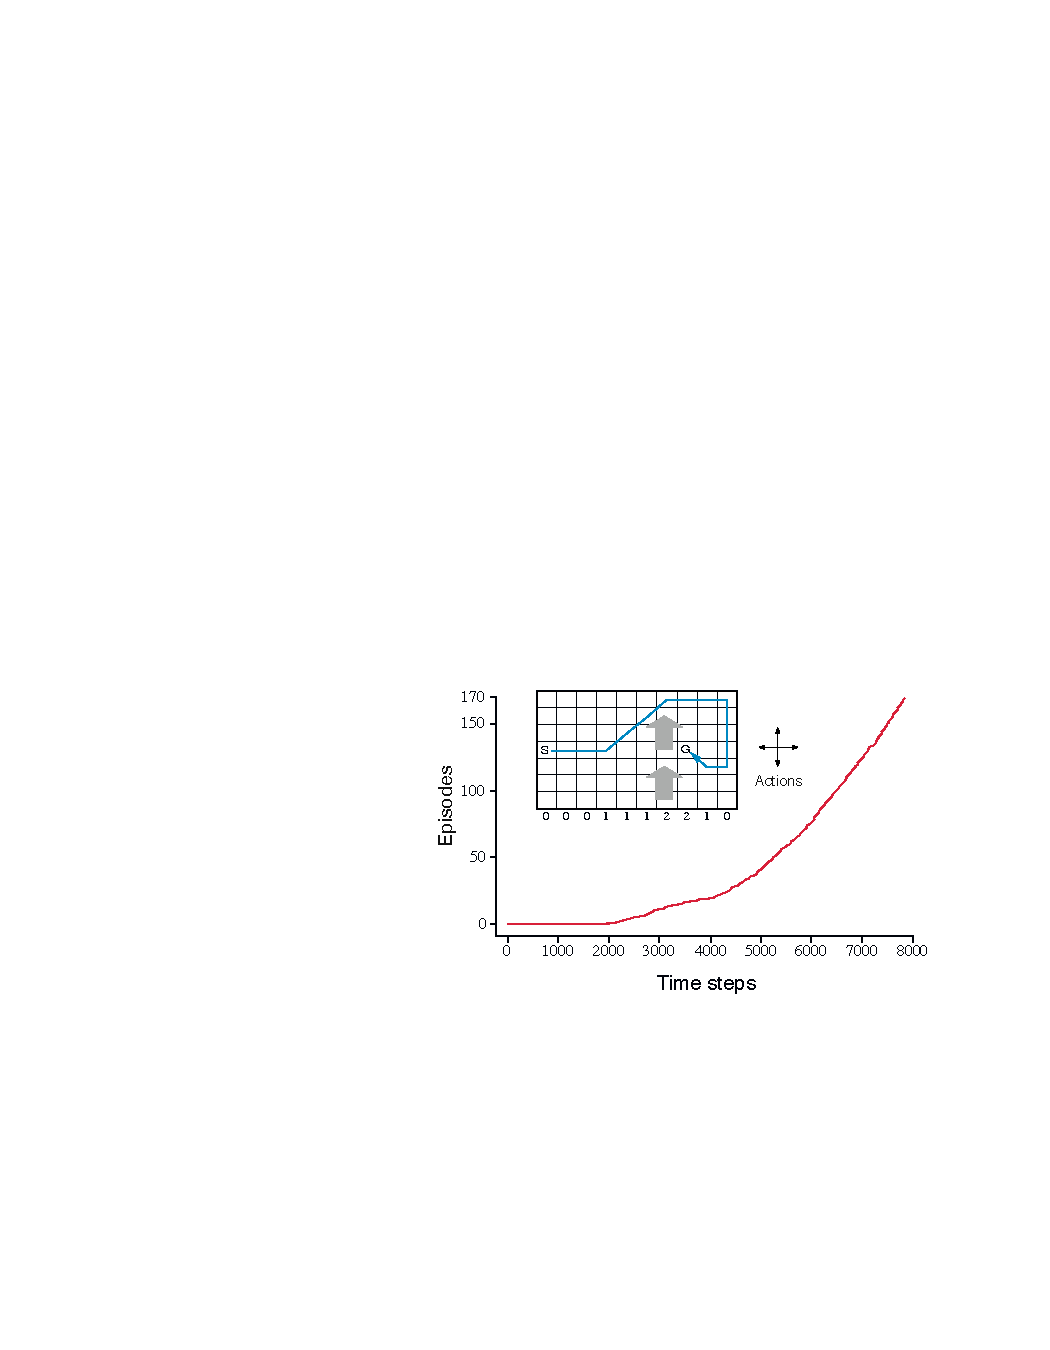
\includegraphics[alt={rlbook 06 12 ex 06_05 windy grid world plot},width=0.75\linewidth]{rlbook-06-12-ex-06_05-windy-grid-world-plot.pdf}
\section{Q-Learning: Off-policy TD Control}
\label{sec:orgc6b36e4}

Sarsa update:

\begin{equation*}
Q(s_t, a_t) \gets Q(s_t, a_t) + \alpha \left[ R_{t+1} + \gamma Q(s_{t+1}, a_{t+1}) - Q(S_t, A_t) \right]
\end{equation*}

Q-learning update:

\begin{equation*}
Q(s_t, a_t) \gets Q(s_t, a_t) + \alpha \left[ R_{t+1} + \gamma \max_{a} Q(s_{t+1}, a) - Q(S_t, A_t) \right]
\end{equation*}

Q-learning is off-policy because the value update is made using \(\max_a\) rather than the \(a\) recommended by the policy being followed.
\section{Q-Learning Algorithm}
\label{sec:org5f6ba15}


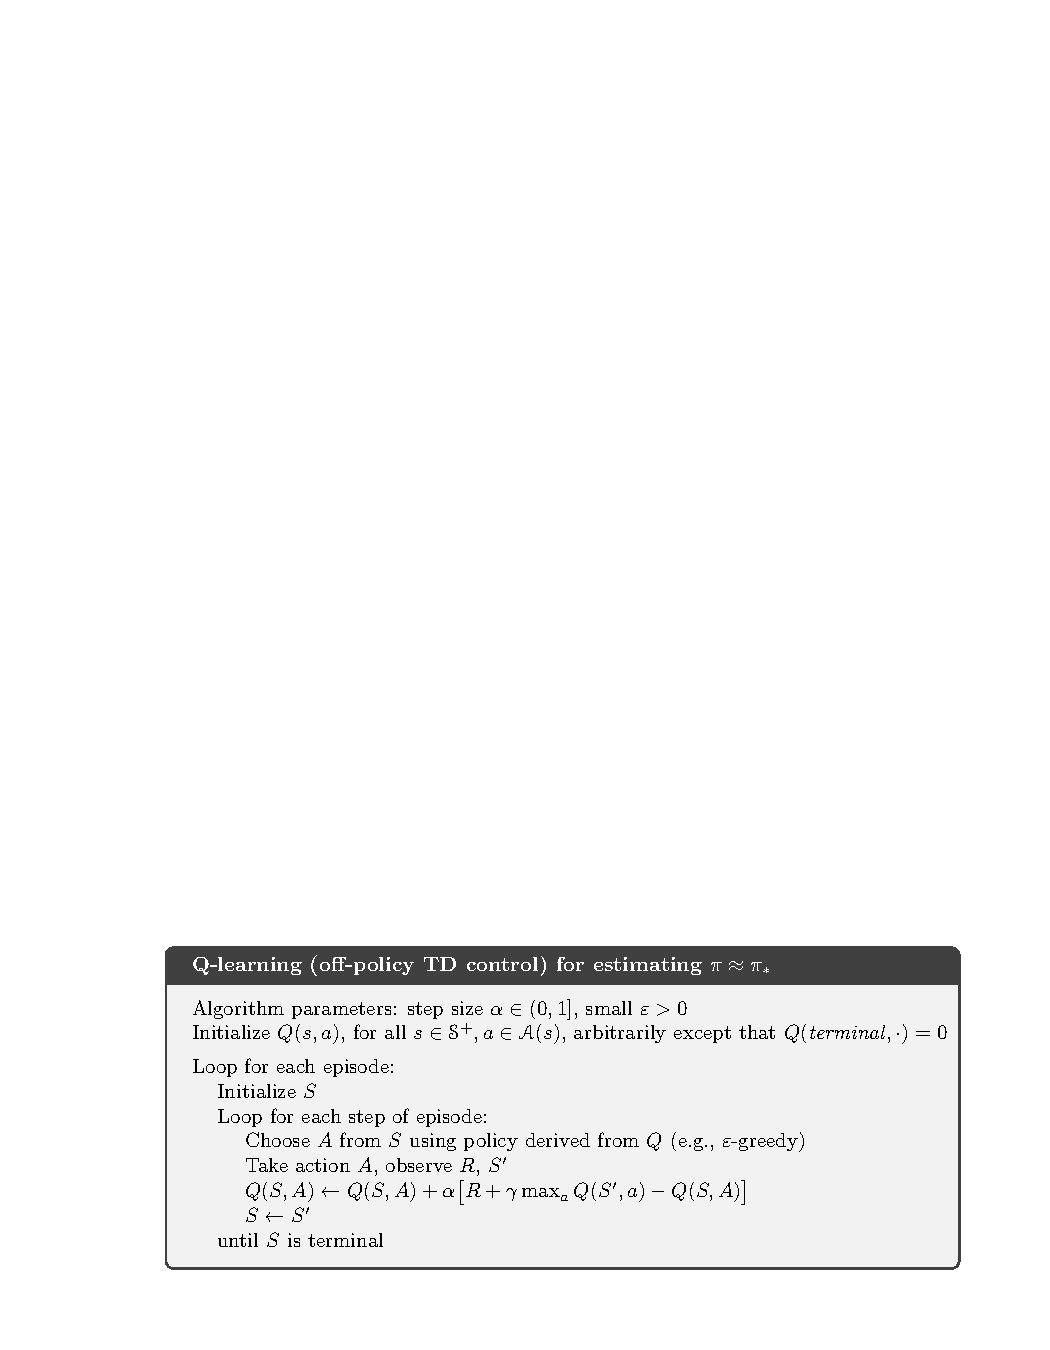
\includegraphics[alt={rlbook 06 13 q learning algorithm},width=0.9\linewidth]{rlbook-06-13-q-learning-algorithm.pdf}
\end{document}
